\documentclass[main.tex]{subfiles}

\begin{document}

\begin{q}{1}
Consider the planet Mars. Calculate its relative distance by using the following observational data. Do not use Kepler's laws of plaentary motion and Newton's law of universal gravitation (assume that they have yet to be discovered).

\noindent\textit{Hint: Consider the reference frame in which the Sun and Earth are not moving. Find the angle subtended at the Sun by two of the phenomena. Use trigonometry to calculate Mars' relative distance.}

\begin{table}[h!]
    \centering
    \begin{tabular}{|c|c|}
    \hline
    \textbf{Date} & \textbf{Phenomenon} \\
    \hline
    2023-11-18 & Conjunction \\
    2024-10-14 & Western quadrature \\
    2025-01-16 & Opposition \\
    2025-04-21 & Eastern quadrature \\
    \hline
    \end{tabular}
    \caption*{Reference: \href{https://eco.mtk.nao.ac.jp/cgi-bin/koyomi/cande/phenomena_en.cgi}{https://eco.mtk.nao.ac.jp/cgi-bin/koyomi/cande/phenomena\_en.cgi}}
    \end{table}
\end{q}

\begin{sol}
First, we define the average distance the Earth and Mars are from the Sun as $1$ and $x$ astronomical unit(s) respectively where $x > 1$. Assuming that the orbits of Earth and Mars around the Sun is perfectly circular, we obtain the following geometric construction.
\begin{figure}[h!]
    \centering
    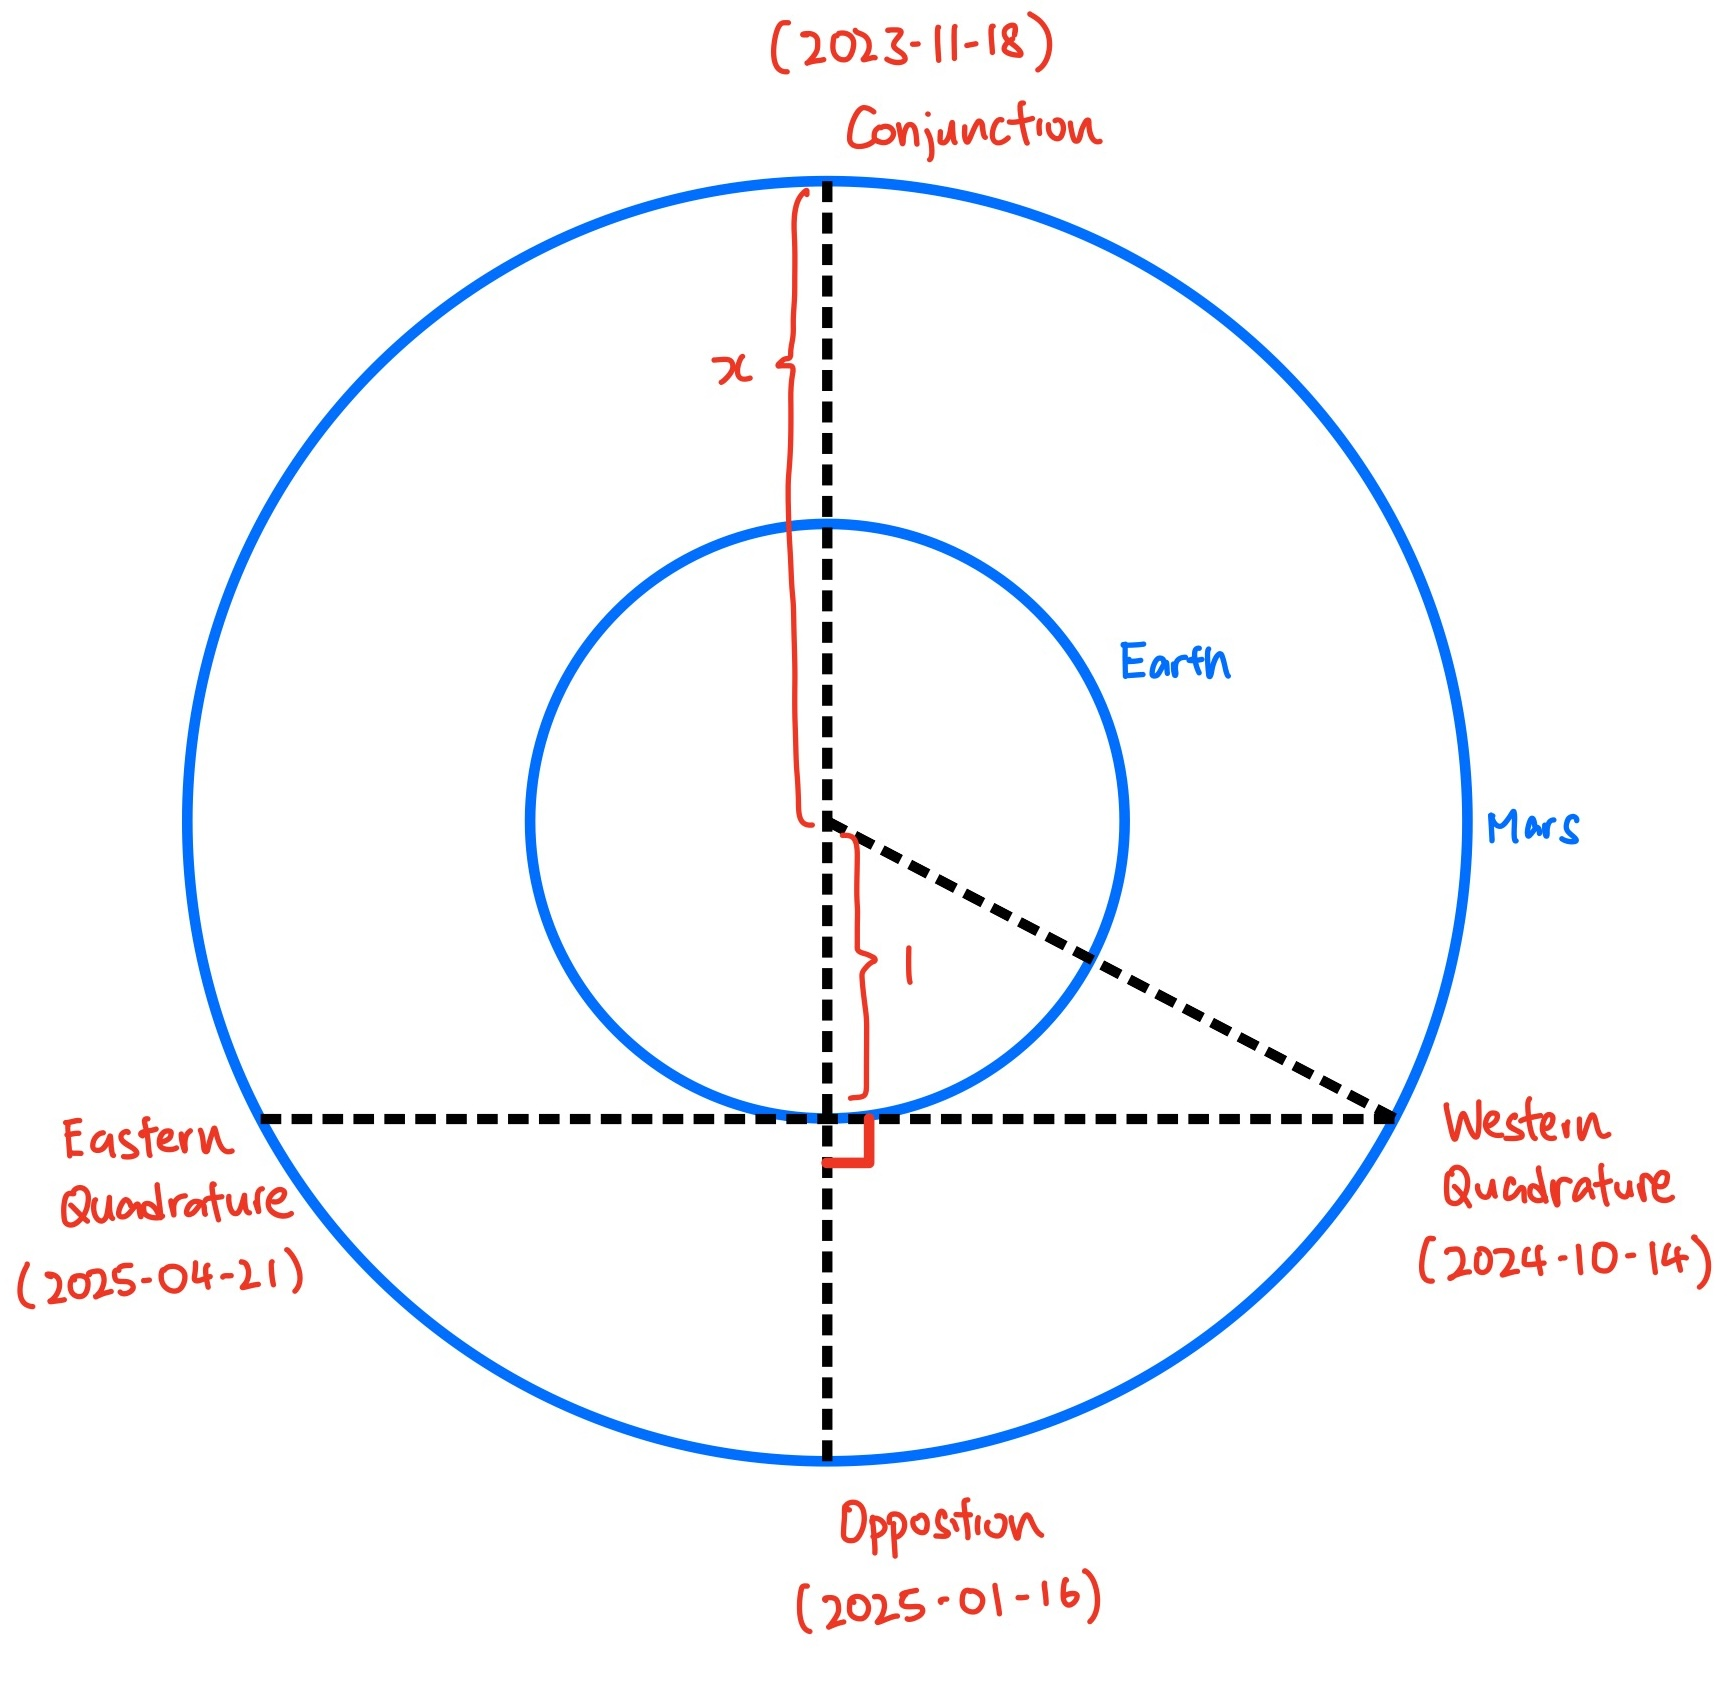
\includegraphics[width=0.5\textwidth]{figure1}
\end{figure}
\newpage\noindent
Where we define $\theta$ as the angle subtended between the Sun-Mars line when Mars is at conjunction (time $t_{\text{conjunction}}$) and the Sun-Mars line when Mars is at time $t$. As such,
\begin{equation}
    \begin{dcases}
        ~\theta\paren{\text{2023-11-18}} = 0 \\
        ~\theta\paren{\text{2025-01-16}} = \frac{\pi}{2}
    \end{dcases}.
\end{equation}
Given the times at where Mars is in conjunction and opposition from Earth, we can obtain the synodic period of Mars as seen from Earth is
\begin{equation}
    t_{\text{synodic}} = 2\sparen{t\paren{\text{2025-01-16}} - t\paren{\text{2023-11-18}}} = \SI{425}{\day}
\end{equation}
Additionally, we define the angle subtended between the Sun-Mars line when Mars is at opposition (time $t_{\text{opposition}}$) and the Sun-Mars line when Mars is at Eastern/Western quadrature (time $t_{\text{eastern quadrature}}$/$t_{\text{western quadrature}}$) as $\varphi$. As such,
\begin{equation}
    \begin{dcases}
        ~\varphi\paren{\text{2024-10-14}} = \frac{\pi}{2} - \varphi \\
        ~\varphi\paren{\text{2025-04-21}} = \frac{\pi}{2} + \varphi
    \end{dcases}.
\end{equation}
Assuming that the 
\end{sol}

\end{document}
